
%% bare_conf.tex
%% V1.3
%% 2007/01/11
%% by Michael Shell

%% http://www.michaelshell.org/
%% for current contact information.
%%
%% This is a skeleton file demonstrating the use of IEEEtran.cls
%% (requires IEEEtran.cls version 1.7 or later) with an IEEE conference paper.
%%
%% Support sites:
%% http://www.michaelshell.org/tex/ieeetran/
%% http://www.ctan.org/tex-archive/macros/latex/contrib/IEEEtran/
%% and
%% http://www.ieee.org/

%%*************************************************************************
%% Legal Notice:
%% This code is offered as-is without any warranty either expressed or
%% implied; without even the implied warranty of MERCHANTABILITY or
%% FITNESS FOR A PARTICULAR PURPOSE! 
%% User assumes all risk.
%% In no event shall IEEE or any contributor to this code be liable for
%% any damages or losses, including, but not limited to, incidental,
%% consequential, or any other damages, resulting from the use or misuse
%% of any information contained here.
%%
%% All comments are the opinions of their respective authors and are not
%% necessarily endorsed by the IEEE.
%%
%% This work is distributed under the LaTeX Project Public License (LPPL)
%% ( http://www.latex-project.org/ ) version 1.3, and may be freely used,
%% distributed and modified. A copy of the LPPL, version 1.3, is included
%% in the base LaTeX documentation of all distributions of LaTeX released
%% 2003/12/01 or later.
%% Retain all contribution notices and credits.
%% ** Modified files should be clearly indicated as such, including  **
%% ** renaming them and changing author support contact information. **
%%
%% File list of work: IEEEtran.cls, IEEEtran_HOWTO.pdf, bare_adv.tex,
%%                    bare_conf.tex, bare_jrnl.tex, bare_jrnl_compsoc.tex
%%*************************************************************************

% *** Authors should verify (and, if needed, correct) their LaTeX system  ***
% *** with the testflow diagnostic prior to trusting their LaTeX platform ***
% *** with production work. IEEE's font choices can trigger bugs that do  ***
% *** not appear when using other class files.                            ***
% The testflow support page is at:
% http://www.michaelshell.org/tex/testflow/



% Note that the a4paper option is mainly intended so that authors in
% countries using A4 can easily print to A4 and see how their papers will
% look in print - the typesetting of the document will not typically be
% affected with changes in paper size (but the bottom and side margins will).
% Use the testflow package mentioned above to verify correct handling of
% both paper sizes by the user's LaTeX system.
%
% Also note that the "draftcls" or "draftclsnofoot", not "draft", option
% should be used if it is desired that the figures are to be displayed in
% draft mode.
%
\documentclass[conference]{IEEEtran}
\usepackage{blindtext, graphicx, subfigure}
% Add the compsoc option for Computer Society conferences.
%
% If IEEEtran.cls has not been installed into the LaTeX system files,
% manually specify the path to it like:
% \documentclass[conference]{../sty/IEEEtran}





% Some very useful LaTeX packages include:
% (uncomment the ones you want to load)


% *** MISC UTILITY PACKAGES ***
%
%\usepackage{ifpdf}
% Heiko Oberdiek's ifpdf.sty is very useful if you need conditional
% compilation based on whether the output is pdf or dvi.
% usage:
% \ifpdf
%   % pdf code
% \else
%   % dvi code
% \fi
% The latest version of ifpdf.sty can be obtained from:
% http://www.ctan.org/tex-archive/macros/latex/contrib/oberdiek/
% Also, note that IEEEtran.cls V1.7 and later provides a builtin
% \ifCLASSINFOpdf conditional that works the same way.
% When switching from latex to pdflatex and vice-versa, the compiler may
% have to be run twice to clear warning/error messages.






% *** CITATION PACKAGES ***
%
%\usepackage{cite}
% cite.sty was written by Donald Arseneau
% V1.6 and later of IEEEtran pre-defines the format of the cite.sty package
% \cite{} output to follow that of IEEE. Loading the cite package will
% result in citation numbers being automatically sorted and properly
% "compressed/ranged". e.g., [1], [9], [2], [7], [5], [6] without using
% cite.sty will become [1], [2], [5]--[7], [9] using cite.sty. cite.sty's
% \cite will automatically add leading space, if needed. Use cite.sty's
% noadjust option (cite.sty V3.8 and later) if you want to turn this off.
% cite.sty is already installed on most LaTeX systems. Be sure and use
% version 4.0 (2003-05-27) and later if using hyperref.sty. cite.sty does
% not currently provide for hyperlinked citations.
% The latest version can be obtained at:
% http://www.ctan.org/tex-archive/macros/latex/contrib/cite/
% The documentation is contained in the cite.sty file itself.






% *** GRAPHICS RELATED PACKAGES ***
%
\ifCLASSINFOpdf
  % \usepackage[pdftex]{graphicx}
  % declare the path(s) where your graphic files are
  % \graphicspath{{../pdf/}{../jpeg/}}
  % and their extensions so you won't have to specify these with
  % every instance of \includegraphics
  % \DeclareGraphicsExtensions{.pdf,.jpeg,.png}
\else
  % or other class option (dvipsone, dvipdf, if not using dvips). graphicx
  % will default to the driver specified in the system graphics.cfg if no
  % driver is specified.
  % \usepackage[dvips]{graphicx}
  % declare the path(s) where your graphic files are
  % \graphicspath{{../eps/}}
  % and their extensions so you won't have to specify these with
  % every instance of \includegraphics
  % \DeclareGraphicsExtensions{.eps}
\fi
% graphicx was written by David Carlisle and Sebastian Rahtz. It is
% required if you want graphics, photos, etc. graphicx.sty is already
% installed on most LaTeX systems. The latest version and documentation can
% be obtained at: 
% http://www.ctan.org/tex-archive/macros/latex/required/graphics/
% Another good source of documentation is "Using Imported Graphics in
% LaTeX2e" by Keith Reckdahl which can be found as epslatex.ps or
% epslatex.pdf at: http://www.ctan.org/tex-archive/info/
%
% latex, and pdflatex in dvi mode, support graphics in encapsulated
% postscript (.eps) format. pdflatex in pdf mode supports graphics
% in .pdf, .jpeg, .png and .mps (metapost) formats. Users should ensure
% that all non-photo figures use a vector format (.eps, .pdf, .mps) and
% not a bitmapped formats (.jpeg, .png). IEEE frowns on bitmapped formats
% which can result in "jaggedy"/blurry rendering of lines and letters as
% well as large increases in file sizes.
%
% You can find documentation about the pdfTeX application at:
% http://www.tug.org/applications/pdftex





% *** MATH PACKAGES ***
%
%\usepackage[cmex10]{amsmath}
% A popular package from the American Mathematical Society that provides
% many useful and powerful commands for dealing with mathematics. If using
% it, be sure to load this package with the cmex10 option to ensure that
% only type 1 fonts will utilized at all point sizes. Without this option,
% it is possible that some math symbols, particularly those within
% footnotes, will be rendered in bitmap form which will result in a
% document that can not be IEEE Xplore compliant!
%
% Also, note that the amsmath package sets \interdisplaylinepenalty to 10000
% thus preventing page breaks from occurring within multiline equations. Use:
%\interdisplaylinepenalty=2500
% after loading amsmath to restore such page breaks as IEEEtran.cls normally
% does. amsmath.sty is already installed on most LaTeX systems. The latest
% version and documentation can be obtained at:
% http://www.ctan.org/tex-archive/macros/latex/required/amslatex/math/





% *** SPECIALIZED LIST PACKAGES ***
%
\usepackage{algorithmic}
% algorithmic.sty was written by Peter Williams and Rogerio Brito.
% This package provides an algorithmic environment fo describing algorithms.
% You can use the algorithmic environment in-text or within a figure
% environment to provide for a floating algorithm. Do NOT use the algorithm
% floating environment provided by algorithm.sty (by the same authors) or
% algorithm2e.sty (by Christophe Fiorio) as IEEE does not use dedicated
% algorithm float types and packages that provide these will not provide
% correct IEEE style captions. The latest version and documentation of
% algorithmic.sty can be obtained at:
% http://www.ctan.org/tex-archive/macros/latex/contrib/algorithms/
% There is also a support site at:
% http://algorithms.berlios.de/index.html
% Also of interest may be the (relatively newer and more customizable)
% algorithmicx.sty package by Szasz Janos:
% http://www.ctan.org/tex-archive/macros/latex/contrib/algorithmicx/




% *** ALIGNMENT PACKAGES ***
%
%\usepackage{array}
% Frank Mittelbach's and David Carlisle's array.sty patches and improves
% the standard LaTeX2e array and tabular environments to provide better
% appearance and additional user controls. As the default LaTeX2e table
% generation code is lacking to the point of almost being broken with
% respect to the quality of the end results, all users are strongly
% advised to use an enhanced (at the very least that provided by array.sty)
% set of table tools. array.sty is already installed on most systems. The
% latest version and documentation can be obtained at:
% http://www.ctan.org/tex-archive/macros/latex/required/tools/


%\usepackage{mdwmath}
%\usepackage{mdwtab}
% Also highly recommended is Mark Wooding's extremely powerful MDW tools,
% especially mdwmath.sty and mdwtab.sty which are used to format equations
% and tables, respectively. The MDWtools set is already installed on most
% LaTeX systems. The lastest version and documentation is available at:
% http://www.ctan.org/tex-archive/macros/latex/contrib/mdwtools/


% IEEEtran contains the IEEEeqnarray family of commands that can be used to
% generate multiline equations as well as matrices, tables, etc., of high
% quality.


%\usepackage{eqparbox}
% Also of notable interest is Scott Pakin's eqparbox package for creating
% (automatically sized) equal width boxes - aka "natural width parboxes".
% Available at:
% http://www.ctan.org/tex-archive/macros/latex/contrib/eqparbox/





% *** SUBFIGURE PACKAGES ***
%\usepackage[tight,footnotesize]{subfigure}
% subfigure.sty was written by Steven Douglas Cochran. This package makes it
% easy to put subfigures in your figures. e.g., "Figure 1a and 1b". For IEEE
% work, it is a good idea to load it with the tight package option to reduce
% the amount of white space around the subfigures. subfigure.sty is already
% installed on most LaTeX systems. The latest version and documentation can
% be obtained at:
% http://www.ctan.org/tex-archive/obsolete/macros/latex/contrib/subfigure/
% subfigure.sty has been superceeded by subfig.sty.



%\usepackage[caption=false]{caption}

%\usepackage[font=footnotesize]{subfig}

% subfig.sty, also written by Steven Douglas Cochran, is the modern
% replacement for subfigure.sty. However, subfig.sty requires and
% automatically loads Axel Sommerfeldt's caption.sty which will override
% IEEEtran.cls handling of captions and this will result in nonIEEE style
% figure/table captions. To prevent this problem, be sure and preload
% caption.sty with its "caption=false" package option. This is will preserve
% IEEEtran.cls handing of captions. Version 1.3 (2005/06/28) and later 
% (recommended due to many improvements over 1.2) of subfig.sty supports
% the caption=false option directly:
%\usepackage[caption=false,font=footnotesize]{subfig}
%
% The latest version and documentation can be obtained at:
% http://www.ctan.org/tex-archive/macros/latex/contrib/subfig/
% The latest version and documentation of caption.sty can be obtained at:
% http://www.ctan.org/tex-archive/macros/latex/contrib/caption/




% *** FLOAT PACKAGES ***
%
%\usepackage{fixltx2e}
% fixltx2e, the successor to the earlier fix2col.sty, was written by
% Frank Mittelbach and David Carlisle. This package corrects a few problems
% in the LaTeX2e kernel, the most notable of which is that in current
% LaTeX2e releases, the ordering of single and double column floats is not
% guaranteed to be preserved. Thus, an unpatched LaTeX2e can allow a
% single column figure to be placed prior to an earlier double column
% figure. The latest version and documentation can be found at:
% http://www.ctan.org/tex-archive/macros/latex/base/



%\usepackage{stfloats}
% stfloats.sty was written by Sigitas Tolusis. This package gives LaTeX2e
% the ability to do double column floats at the bottom of the page as well
% as the top. (e.g., "\begin{figure*}[!b]" is not normally possible in
% LaTeX2e). It also provides a command:
%\fnbelowfloat
% to enable the placement of footnotes below bottom floats (the standard
% LaTeX2e kernel puts them above bottom floats). This is an invasive package
% which rewrites many portions of the LaTeX2e float routines. It may not work
% with other packages that modify the LaTeX2e float routines. The latest
% version and documentation can be obtained at:
% http://www.ctan.org/tex-archive/macros/latex/contrib/sttools/
% Documentation is contained in the stfloats.sty comments as well as in the
% presfull.pdf file. Do not use the stfloats baselinefloat ability as IEEE
% does not allow \baselineskip to stretch. Authors submitting work to the
% IEEE should note that IEEE rarely uses double column equations and
% that authors should try to avoid such use. Do not be tempted to use the
% cuted.sty or midfloat.sty packages (also by Sigitas Tolusis) as IEEE does
% not format its papers in such ways.





% *** PDF, URL AND HYPERLINK PACKAGES ***
%
%\usepackage{url}
% url.sty was written by Donald Arseneau. It provides better support for
% handling and breaking URLs. url.sty is already installed on most LaTeX
% systems. The latest version can be obtained at:
% http://www.ctan.org/tex-archive/macros/latex/contrib/misc/
% Read the url.sty source comments for usage information. Basically,
% \url{my_url_here}.





% *** Do not adjust lengths that control margins, column widths, etc. ***
% *** Do not use packages that alter fonts (such as pslatex).         ***
% There should be no need to do such things with IEEEtran.cls V1.6 and later.
% (Unless specifically asked to do so by the journal or conference you plan
% to submit to, of course. )


% correct bad hyphenation here
\hyphenation{op-tical net-works semi-conduc-tor}


\begin{document}
%
% paper title
% can use linebreaks \\ within to get better formatting as desired
\title{A Resilient DAP Dynamic Selection Algorithm Based on Quality Aware Metric for Smart Grids}


% author names and affiliations
% use a multiple column layout for up to three different
% affiliations
\author{\IEEEauthorblockN{Victor Hugo Okabayashi}
\IEEEauthorblockA{Instituto de Computa\c{c}\~ ao\\Universidade Federal Fluminense(UFF)\\Niter\' oi, RJ, Brasil\\
Email: vhugo@ic.uff.br}
\and
\IEEEauthorblockN{ Diego Passos}
\IEEEauthorblockA{Instituto de Computa\c{c}\~ ao\\Universidade Federal Fluminense(UFF)\\Niter\' oi, RJ, Brasil\\
Email: dpassos@ic.uff.br}
\and
\IEEEauthorblockN{C\' elio V. N. Albuquerque\\ Instituto de Computa\c{c}\~ ao\\Universidade Federal Fluminense(UFF)\\Niter\' oi, RJ, Brasil\\
Email: celio@ic.uff.br}}

% conference papers do not typically use \thanks and this command
% is locked out in conference mode. If really needed, such as for
% the acknowledgment of grants, issue a \IEEEoverridecommandlockouts
% after \documentclass

% for over three affiliations, or if they all won't fit within the width
% of the page, use this alternative format:
% 
%\author{\IEEEauthorblockN{Michael Shell\IEEEauthorrefmark{1},
%Homer Simpson\IEEEauthorrefmark{2},
%James Kirk\IEEEauthorrefmark{3}, 
%Montgomery Scott\IEEEauthorrefmark{3} and
%Eldon Tyrell\IEEEauthorrefmark{4}}
%\IEEEauthorblockA{\IEEEauthorrefmark{1}School of Electrical and Computer Engineering\\
%Georgia Institute of Technology,
%Atlanta, Georgia 30332--0250\\ Email: see http://www.michaelshell.org/contact.html}
%\IEEEauthorblockA{\IEEEauthorrefmark{2}Twentieth Century Fox, Springfield, USA\\
%Email: homer@thesimpsons.com}
%\IEEEauthorblockA{\IEEEauthorrefmark{3}Starfleet Academy, San Francisco, California 96678-2391\\
%Telephone: (800) 555--1212, Fax: (888) 555--1212}
%\IEEEauthorblockA{\IEEEauthorrefmark{4}Tyrell Inc., 123 Replicant Street, Los Angeles, California 90210--4321}}




% use for special paper notices
%\IEEEspecialpapernotice{(Invited Paper)}




% make the title area
\maketitle


\begin{abstract}
%\boldmath
  Smart Grids are the evolution of the current electric system to meet the challenge of increasing demands for energy in this century by integrating the eletric grid with data communication network. The challenge of this network is to fulfill safety requirements: reliability and resilience required in order to meet various types of services and applications. The use of wireless mesh networks can provide scalability and resilience to this communication network, but there are challenges that need to be evaluated and analyzed so that it is in fact a solution for communications in Smart Grids. This paper proposes an algorithm for dynamic selection of gateways in a muultihoming Smart Grid network improving performance when a gateway's fault occurs on congested environments. The results indicate that the proposed algorithm makes the routing protocol more robust and resilient against ......
\end{abstract}
% IEEEtran.cls defaults to using nonbold math in the Abstract.
% This preserves the distinction between vectors and scalars. However,
% if the journal you are submitting to favors bold math in the abstract,
% then you can use LaTeX's standard command \boldmath at the very start
% of the abstract to achieve this. Many IEEE journals frown on math
% in the abstract anyway.

% Note that keywords are not normally used for peerreview papers.
\begin{IEEEkeywords}
reliability, smart grid, wireless mesh networks (WMNs).

\end{IEEEkeywords}






% For peer review papers, you can put extra information on the cover
% page as needed:
% \ifCLASSOPTIONpeerreview
% \begin{center} \bfseries EDICS Category: 3-BBND \end{center}
% \fi
%
% For peerreview papers, this IEEEtran command inserts a page break and
% creates the second title. It will be ignored for other modes.
\IEEEpeerreviewmaketitle



\section{Introduction}
Basically the current electrical system has an outdated hierarchical architecture that does not meet the future demands of energy consumption due to various limitations such as limited generation capacity, one-way flow of energy (generation–transport–distribution–consumption) and communication,  low and deficient communication, the use of fossil fuels in power generation and reliability problems \cite{Farhangi2010}. 
Modernization the existing electricity grid aims to solve these problems, improving efficiency, reliability and security, integrating the use of renewable energy produced by consumers, making the one-way flow in two-way flow for energy and communication \cite {Farhangi2010,Moslehi2010}. Two-way communication infrastructure is essential for Smart Grids \cite{Gungor2011}, cause it needs to send commands and to receive information from its components and sensors  in real time, with reliably, allowing monitoring, maintenance and control of the entire grid. 

Smart Grids require two-way communication that has specificities of delay, bandwidth, frequency of updates, reliability, security and time response for each distinct application in their different fields \cite{Gungor2011}. Advanced Metering Infrastructure (AMI) is fundamental and the first step to realize a Smart Grid\cite{4781067,5484223}. Your security requirements should provide robustness and resilience to prevent or recover from cyber attacks or problems caused by interference, providing the stability and reliability to AMI communication. This communication may use available wired or wireless technologies that support the exchange information between components of AMI \cite{Saputro2012,4547164}. Different types of technologies can be used: cellular technology \cite{5589988}, WiMAX, ZigBee \cite{5589988}, RF Mesh \cite{5622071}, IEEE 802.11-based Wireless Mesh Networks (WMN) and PLC \cite{5479945}. 

PLC (\emph{Power Line Communication}) is the most used wired technology \cite{Saputro2012}, but has limitations. In case of failures, such as physical disruption of power lines, would not be possible to maintain communication between AMI components \cite{Gungor2006}. Wireless networks offer more benefits than wired networks such as lower cost, ease of deployment and the available signal in a large area \cite{5589988}. Among all wireless technologies WMN has advantages compared to single-hop infrastructure network architecture, because it communicates in multi-hop way that extends the coverage of the network and allowing communication with alternative paths in case of failures in links \cite{5622071,Fang2012}. 

The challenge is to adapt WMN to communication requirements required by AMI, where hundreds of meters communicate with Utility's head-end through DAP (Data Aggregation Point), which are the gateways of this network. This large number of nodes is the main challenge for the WMN \cite{Akyildiz2005}, since more than 100 meters may be associated to one DAP. If they  send data simultaneously should cause congestion to the network. A way to reduce this problem is the use of multiple DAP. There are other problems related to the propagation conditions of the external environment that provide attenuation, interference and variation to the signal strength \cite{Gungor2011}. The routing protocol must be able to find reliable routes to improve performance and meet the requirements of AMI network.

The new wireless communication devices have the capacity to operate in different transmission rates and are sensitive to propagation conditions generating another challenge for routing and its metric. The latter should take into account the fluctuations of link quality and transmission
rate for consistent assessment of costs.

Given the problems faced by routing protocol in WMN to comply with AMI communication requirements, we propose an algorithm that dynamically selects a DAP for communication between meters and headend. In this problem, we assumed that each meter can connect, through multiple hops, to a set of DAP. The main goal of this algorithm, called \ emph {DAP} Dynamic Selection Algorithm (DDSA), is to increase the reliability, robustness and resiliency using multiple DAP by meters thus improving performance in a presence of DAP's failure, since there is the probability of choosing other DAP for communication with the headend.

The organization of the paper is as follows. In Section II, discloses the particularities of the AMI communication network and its challenges and problems. Section III presents related work. Section IV describes and explains the working principle of DDSA. Section V presents the results obtained in the simulations. Section VI concludes the paper and presents ideas for future work.


% needed in second column of first page if using \IEEEpubid
%\IEEEpubidadjcol

% An example of a floating figure using the graphicx package.
% Note that \label must occur AFTER (or within) \caption.
% For figures, \caption should occur after the \includegraphics.
% Note that IEEEtran v1.7 and later has special internal code that
% is designed to preserve the operation of \label within \caption
% even when the captionsoff option is in effect. However, because
% of issues like this, it may be the safest practice to put all your
% \label just after \caption rather than within \caption{}.
%
% Reminder: the "draftcls" or "draftclsnofoot", not "draft", class
% option should be used if it is desired that the figures are to be
% displayed while in draft mode.
%
%\begin{figure}[!t]
%\centering
%\includegraphics[width=2.5in]{myfigure}
% where an .eps filename suffix will be assumed under latex, 
% and a .pdf suffix will be assumed for pdflatex; or what has been declared
% via \DeclareGraphicsExtensions.
%\caption{Simulation Results}
%\label{fig_sim}
%\end{figure}

% Note that IEEE typically puts floats only at the top, even when this
% results in a large percentage of a column being occupied by floats.


% An example of a double column floating figure using two subfigures.
% (The subfig.sty package must be loaded for this to work.)
% The subfigure \label commands are set within each subfloat command, the
% \label for the overall figure must come after \caption.
% \hfil must be used as a separator to get equal spacing.
% The subfigure.sty package works much the same way, except \subfigure is
% used instead of \subfloat.
%
%\begin{figure*}[!t]
%\centerline{\subfloat[Case I]\includegraphics[width=2.5in]{subfigcase1}%
%\label{fig_first_case}}
%\hfil
%\subfloat[Case II]{\includegraphics[width=2.5in]{subfigcase2}%
%\label{fig_second_case}}}
%\caption{Simulation results}
%\label{fig_sim}
%\end{figure*}
%
% Note that often IEEE papers with subfigures do not employ subfigure
% captions (using the optional argument to \subfloat), but instead will
% reference/describe all of them (a), (b), etc., within the main caption.


% An example of a floating table. Note that, for IEEE style tables, the 
% \caption command should come BEFORE the table. Table text will default to
% \footnotesize as IEEE normally uses this smaller font for tables.
% The \label must come after \caption as always.
%
%\begin{table}[!t]
%% increase table row spacing, adjust to taste
%\renewcommand{\arraystretch}{1.3}
% if using array.sty, it might be a good idea to tweak the value of
% \extrarowheight as needed to properly center the text within the cells
%\caption{An Example of a Table}
%\label{table_example}
%\centering
%% Some packages, such as MDW tools, offer better commands for making tables
%% than the plain LaTeX2e tabular which is used here.
%\begin{tabular}{|c||c|}
%\hline
%One & Two\\
%\hline
%Three & Four\\
%\hline
%\end{tabular}
%\end{table}


% Note that IEEE does not put floats in the very first column - or typically
% anywhere on the first page for that matter. Also, in-text middle ("here")
% positioning is not used. Most IEEE journals use top floats exclusively.
% Note that, LaTeX2e, unlike IEEE journals, places footnotes above bottom
% floats. This can be corrected via the \fnbelowfloat command of the
% stfloats package.

\section{Background}

\subsection{A Brief Overview of AMI}


The modernization of the current electricity grid involves a large use of information technology to move the current system towards Smart Grid using communication that allows bidirectional flow of information between the different subsystems and the headend. Nearly 8\% of all energy generated is lost along the transmission lines and 20\% of the total generation capacity is only to supply peak demands, which represent only 5\% of the total demand \cite{Farhangi2010}. About 90\% of power outages and disturbances are assigned to distribution subsystem, thus the success of a Smart Grid depends on the deployment of an interconnected distribution subsystem. 

AMI is the main application of distribution subsystem that aims to improve the reliability and  a change in paradigm  to one where customer demand adjusts to the power generation. AMI is basically composed of smart meters, gateways or DAP and  Utility's headend, all interconnected by a communication network. The meters send the measurement data to the headend through DAP and this traffic is characterized by the exchange of short messages.  

These messages have a payload that varies from tens to hundreds of bytes and are sent periodically, typically in a 15 minutes interval, and remain inactive the rest of the time \cite{SRS:13,4547164}. They can be sent in a single data packet originated by meters connected to a DAP. The headend can send commands and requests to meters also through DAP.


\subsection{Problem Statement}

According \cite{Gungor2013}, it is necessary for each meter a band from 10 to 100 Kbps and the latency should be less than 2000 ms. Since investments in the power sector are long-lasting, it is desirable that the AMI should also support long-term operations \cite{5484223}. New necessities for information may arise and making the requirements more stringent such as latency that should be less than hundreds or tens of milliseconds in applications that need information in real time.

The AMI traffic can be classified into regular and on-demand. It's regular when data consumption are automatically sent by the meters at predetermined intervals time \cite{Plan2011,4547164} and constitute the majority of data traffic flowing through AMI \cite{5484223}. The on-demand traffic is constituted of alert messages from meters, command and control sent by the headend  to meters and DAP and the responses to these commands \cite{Plan2011}. In the latter type of traffic can occur a greater increase in network congestion due to the request for sending information,  by  headend to a large numbers of meters, that would send simultaneously this data. DAP is a single point of failure, because all traffic between meters and headend or vice versa flows through it, a failure in it will stop the entire network from working.

The residential density of the area, which can be a dense urban area or rural area, determines the amount of meters per area, which according to \cite{Plan2011} can be classified into rural, suburban or urban scenario, with density varying from 10, 800 or 2000 meters per km\textsuperscript{2}, respectively. The external environment conditions in combination with the number of meter will determine the level of interference and attenuation in communication between meters and DAP will have. This may cause breaks in routes and loss of performance due to the increase in packet loss and retransmissions \cite{farooq2013energy}. 


Due to the peculiarities of the AMI network and a large amount of meters acting as routers/clients mesh, there is a possibility of problems with loops and broken route \cite{ramachandran2007routing}, causing a degradation in performance that may lead to a non-compliance with communication requirements. The density of the WMN varies with the number of households in the region which can be dense or a very sparse area. Thus the routing protocol should handle this variation, providing an acceptable level of service regardless of WMN density. Another problem is the increased amount of collisions near the DAP because all packets are routing to it \cite{Saputro2012}.


\begin{figure*}[ht]
  \centering
  \mbox{
    \subfigure[DDSA-30\label{DDSA-30}]{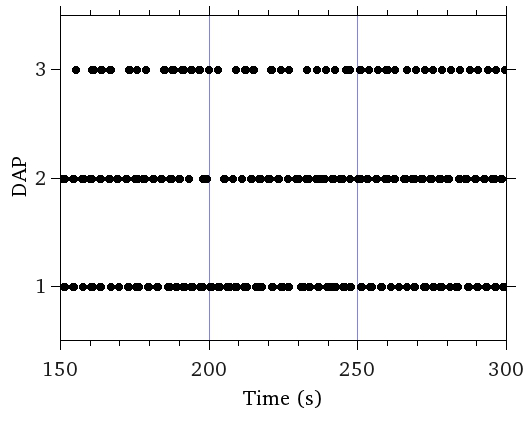
\includegraphics[scale=.35]{IEEE-consolidados/G-troca-gw-ddsa30.jpg}}\quad
    \subfigure[DDSA-85\label{DDSA-85}]{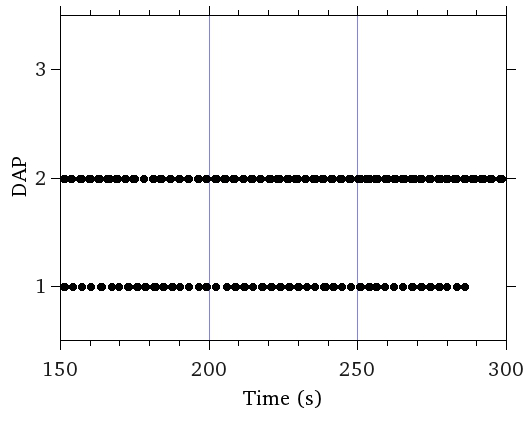
\includegraphics[scale=.35]{IEEE-consolidados/G-troca-gw-ddsa85.jpg}}\quad
    \subfigure[Multi-DAP\label{Multi-DAP}]{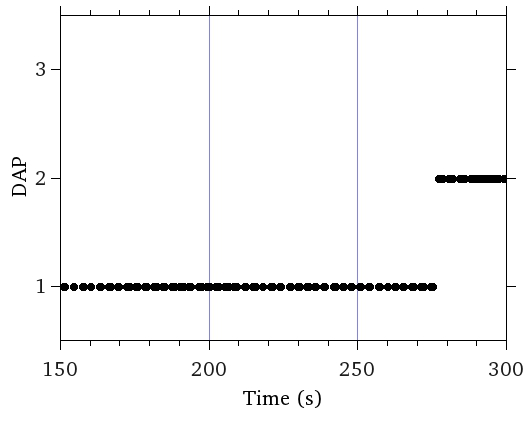
\includegraphics[scale=.35]{IEEE-consolidados/G-troca-gw-multidap.jpg}}
  }
  \caption{DAP's choice by node 16}
  \label{n16-dap}
\end{figure*}

\begin{figure*}[ht]
  \centering
  \mbox{
    \subfigure[DDSA-30\label{DDSA30-2}]{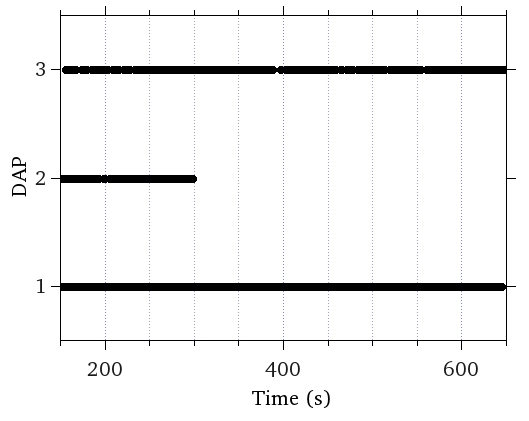
\includegraphics[scale=.35]{IEEE-consolidados/G-troca-gw-ddsa30-2.jpg}}\quad
    \subfigure[DDSA-85\label{DDSA85-2}]{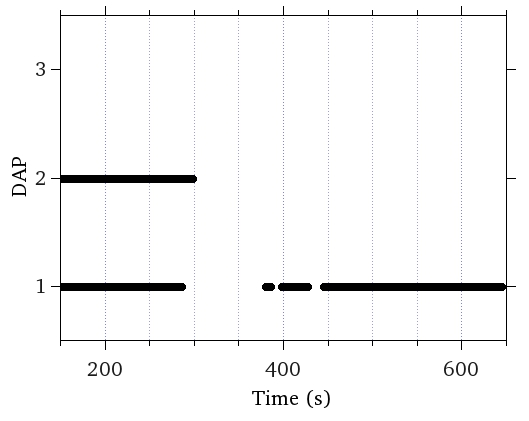
\includegraphics[scale=.35]{IEEE-consolidados/G-troca-gw-ddsa85-2.jpg}}\quad
    \subfigure[Multi-DAP\label{MultiDAP-2}]{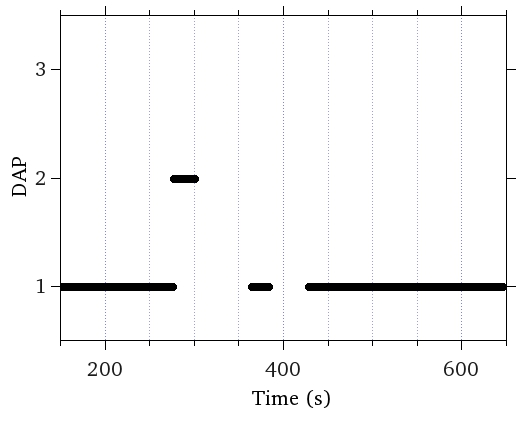
\includegraphics[scale=.35]{IEEE-consolidados/G-troca-gw-multidap-2.jpg}}
  }
  \caption{Packets delivered by node 16}
  \label{n16-dap2}
\end{figure*}


\section{Related Work}

The work in \cite{Gungor2006}  proposes the use of WMN in AMI where multiple domains of mesh networks are connected by a WiMAX backbone. This architecture provides redundant paths between meters eliminating problems like nodes failed and route break increasing their resilience and making network fault tolerant. However, as there is only one DAP acting as gateway in each WMN domain, if it becomes unavailable there will be no communication between the meters and the headend. This is the same problem \cite{Silva2010}, where the WMN consists of meters, routers and collectors. The meters communicate with routers or directly to collectors, the latter controls up to 25,000 meters and routers on a single network.

The work in \cite{Silva2010} makes use of multiple gateways to increase the WMN resilience, cause in addition to providing  providing redundant paths also provides redundancy of gateway.Another work that solves the problem of multiple gateways is \cite{ClaytonR.daSilva2011}  which also preserves the gateway output for each connection, but also adds load balancing. These approaches are applied to WMN that serve as the backbone for internet access. In these access networks is common to use the technique NAT (Network Address Translation), which does not exist in AMI, being necessary to preserve the connection with the gateway output and no breakage of TCP connections semantics occur.

The work in \cite{6412861} and \cite{Gharavi2011} are designed to suit the requirements of AMI networks and make use of multiple DAP for communication between meters and headend modifying the HWMP protocol (Wireless Hybrid mesh Protocol). The work in \cite{Gharavi2011} although solve the problem of discard of the queue, still suffers from other problems such as protocol stability of routes and loops that according to the authors is a characteristic of distributed backpressure system adopted by them. However, neither of them has been evaluated the protocol behavior in an environment with a DAP failure, nor using adaptation of transmission rate, which increases the problem of instability of routes. They use as a base protocol that has scalability problems and congestion caused by control messages \cite{5473885} making it difficult to use in AMI.


Our proposal DDSA makes use of multiple DAP for communication between meters and Central Processing and differs from \cite{6412861} and \cite{Gharavi2011} to be independent of the routing protocol and metric, and can be implemented in that best suit the implementation of AMI and also be designed to improve performance in environments with DAP failure.
In DDSA, each new send data, meters probabilistically choose DAP to which the data packet is sent. 
Thus, improved performance and network security by distributing traffic between the DAP to each transmission, as the probability of selection of each one, and provide resilience as if one is unavailable, it is possible to choose another.


\subsection{Routing Metrics}
 

MARA (Metric-Aware Rate Adaptation) \cite{6051505} is a mechanism that joins routing metric with rate adaptation for transmission in WMN through the concept of cross-layer design.
It uses statistical information of routing metrics to select the best rate and in turn, based on this choice, the metric can estimate the actual cost of the link.
Thus, metrics and rate adaptation share information and make decisions together resulting in better choices of routes by the routing protocol.
The calculation of the metric of a link is based on a conversion process in which first is estimated the SNR (Signal-to-noise ratio) from the link success probability of probe packets in a given transmission rate that can be of 1, 18, 36 or 54 Mbps.
With this SNR estimation is possible, by means of a probability function loss estimate the PER (Packet Error Rate) to other rates. Its advantage is that it solves the problem that metric and choice of rate are studied separately, although they are strongly related.



\section{DDSA (DAP Dynamic Selection Algorithm)}


\section{Performance Evaluation}

\subsection{Simulation Environment}  

\subsection{Simulation Results}


\begin{figure}[ht]
  \centering
  \label{intv-dap}{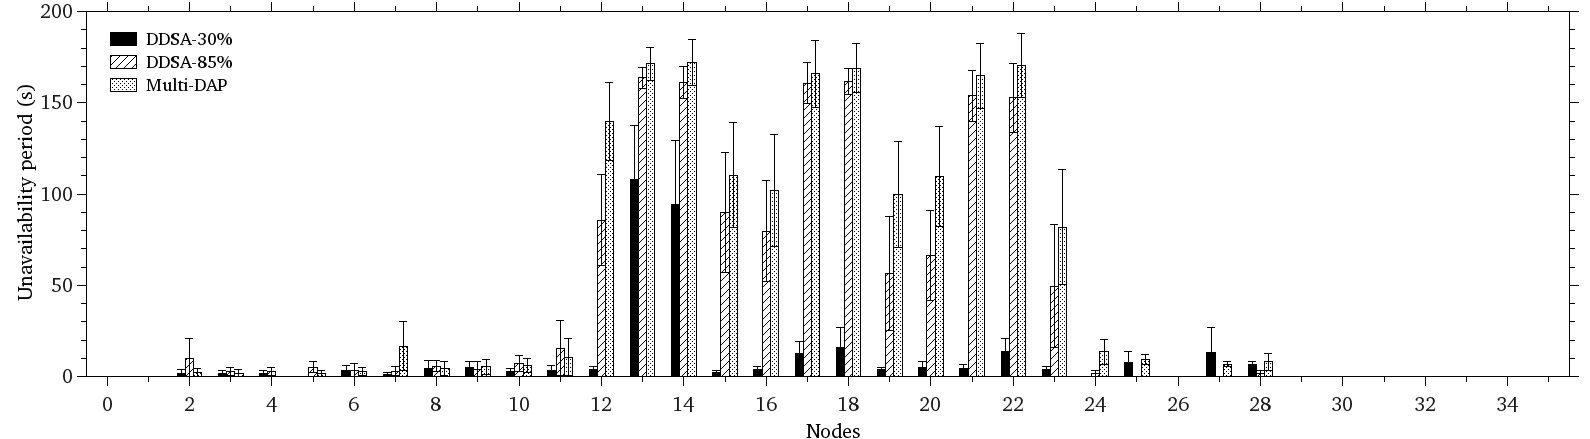
\includegraphics[scale=.21]{IEEE-consolidados/G-wo-rcv-pkt.jpg}} 
  \caption{Sum of intervals without receiving packets in any DAP}
  \label{sum-intv}
\end{figure}


\begin{figure}[ht]
  \centering
  \mbox{
    \label{pdf-n16-per}{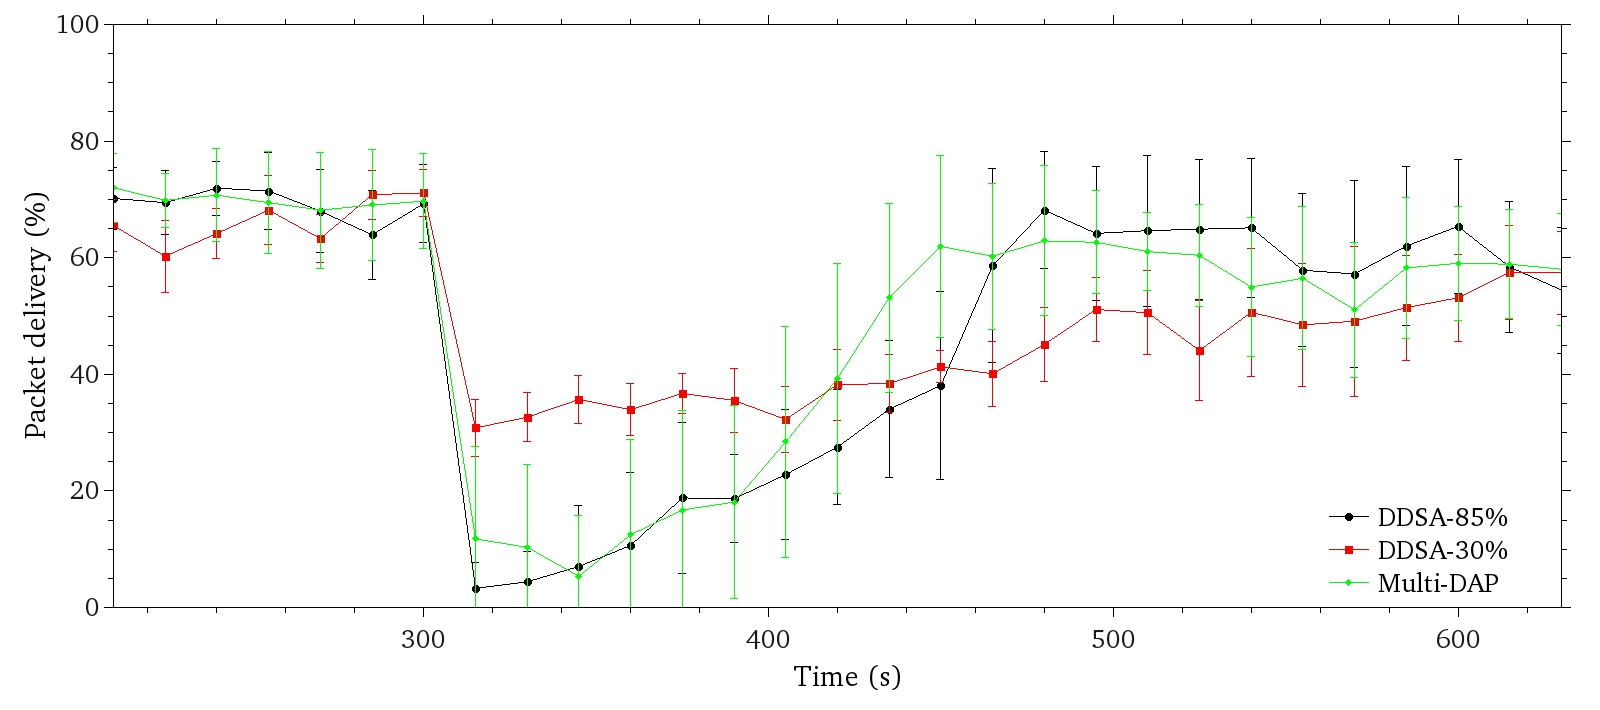
\includegraphics[scale=.21]{IEEE-consolidados/G-pdf-periodo-n16.jpg}}
  }
  \caption{Packet delivery of node 16 in 15 seconds intervals}
  \label{pdf-n16-per}
\end{figure}

\begin{figure}[ht]
  \centering
  \mbox{
    \label{pdf-n16-per}{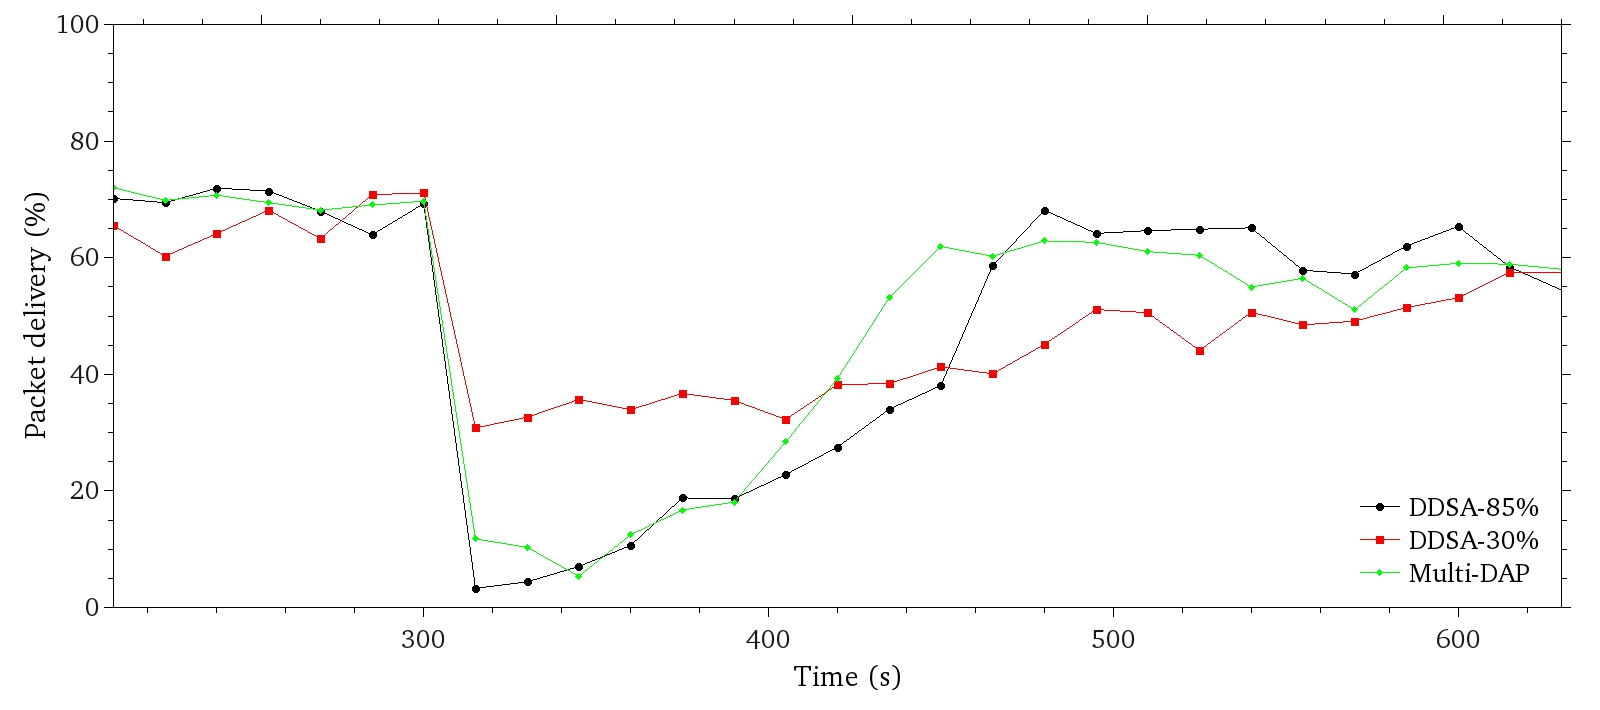
\includegraphics[scale=.21]{IEEE-consolidados/G-pdf-periodo-n16-2.jpg}}
  }
  \caption{Packet delivery of node 16 in 15 seconds intervals}
  \label{pdf-n16-per}
\end{figure}

\begin{figure}[ht]
  \centering
  \mbox{
    \subfigure[all nodes\label{pdf-n16-per}]{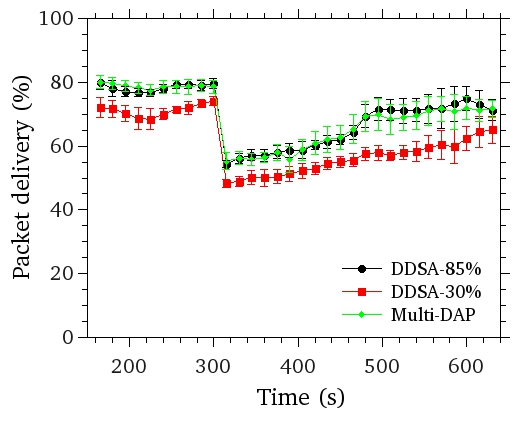
\includegraphics[scale=.33]{IEEE-consolidados/G-todos-periodo.jpg}}
    \subfigure[central nodes (12 to 23)\label{pdf-n16-per}]{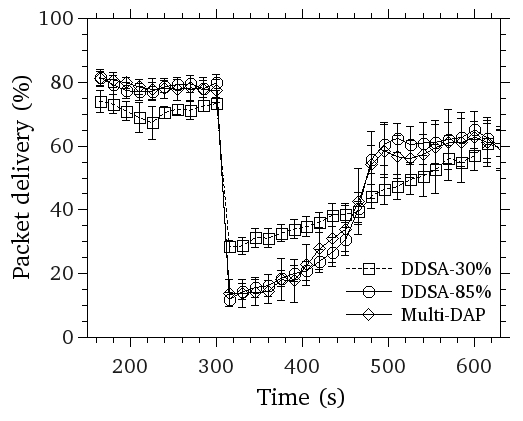
\includegraphics[scale=.33]{IEEE-consolidados/G-centro-periodo.jpg}}
  }
  \caption{Packet delivery in 15 seconds intervals}
  \label{pdf-n16-per}
\end{figure}


\begin  {figure}[ht]
\begin{minipage}[b]{.4\linewidth}
\centering
\subfigure[DDSA-30]
{\label{fase:a}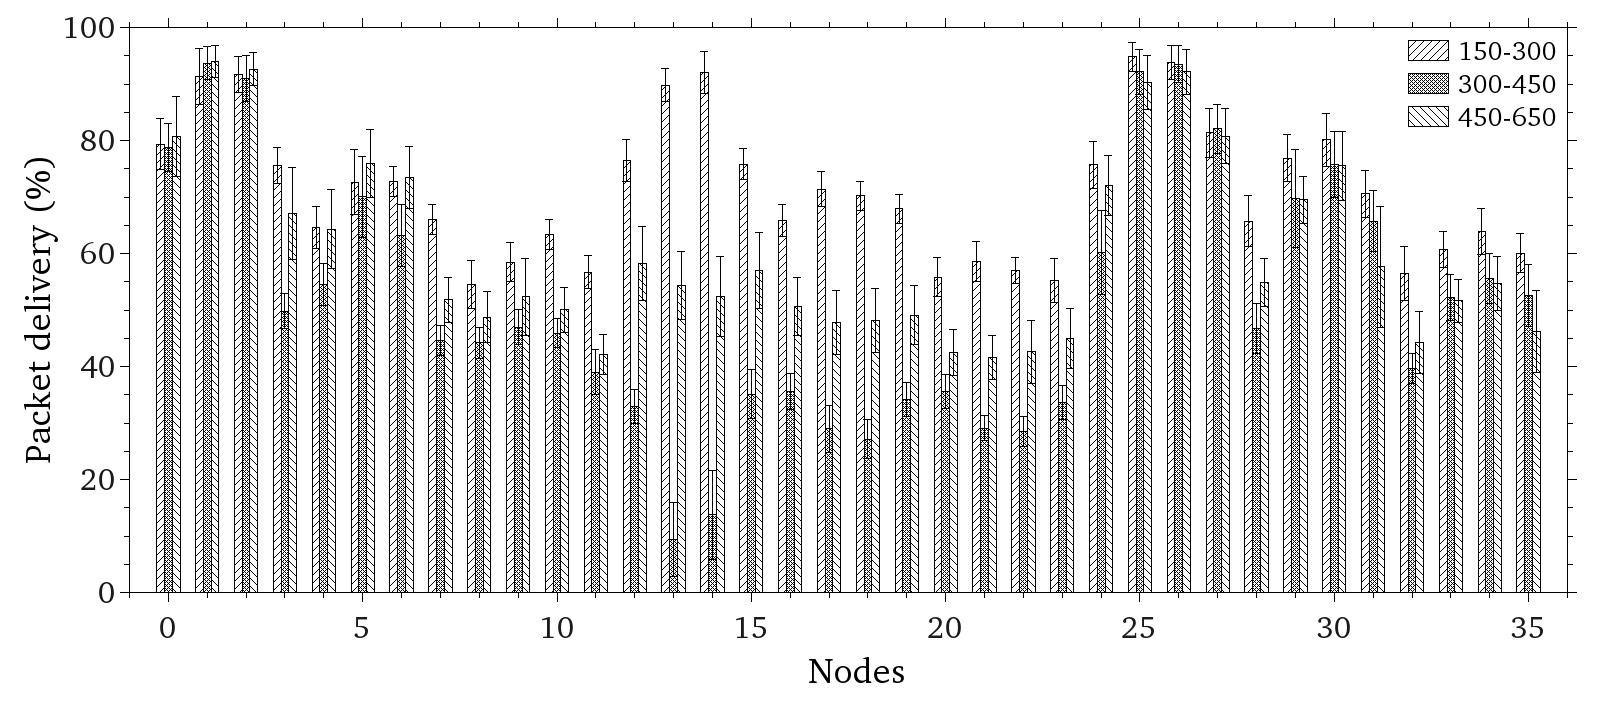
\includegraphics[scale=.21]{IEEE-consolidados/G-no-fases-30.jpg}}

\subfigure[DDSA-85]
{\label{fase:b}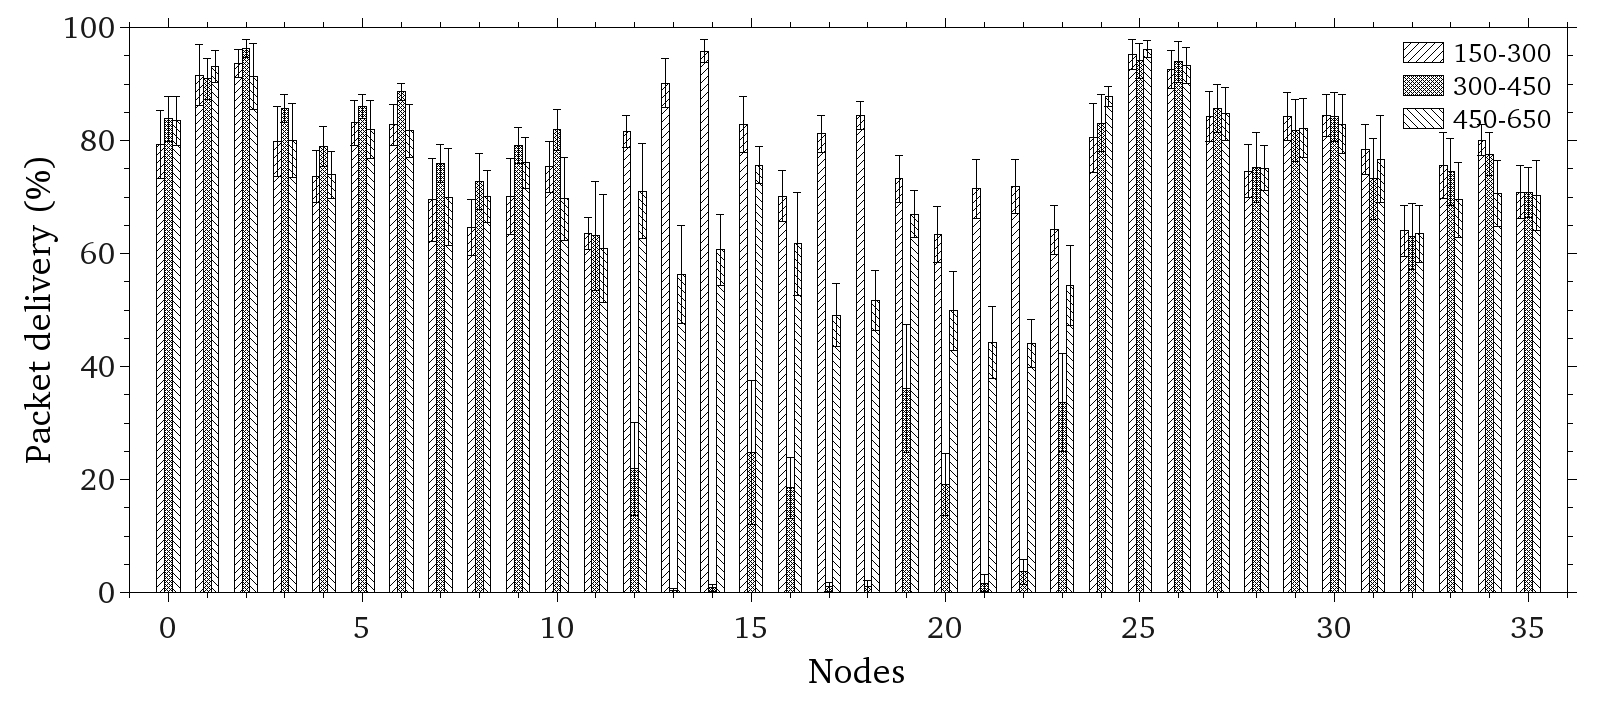
\includegraphics[scale=.21]{IEEE-consolidados/G-no-fases-85.jpg}}

\subfigure[Multi-DAP]
{\label{fase:c}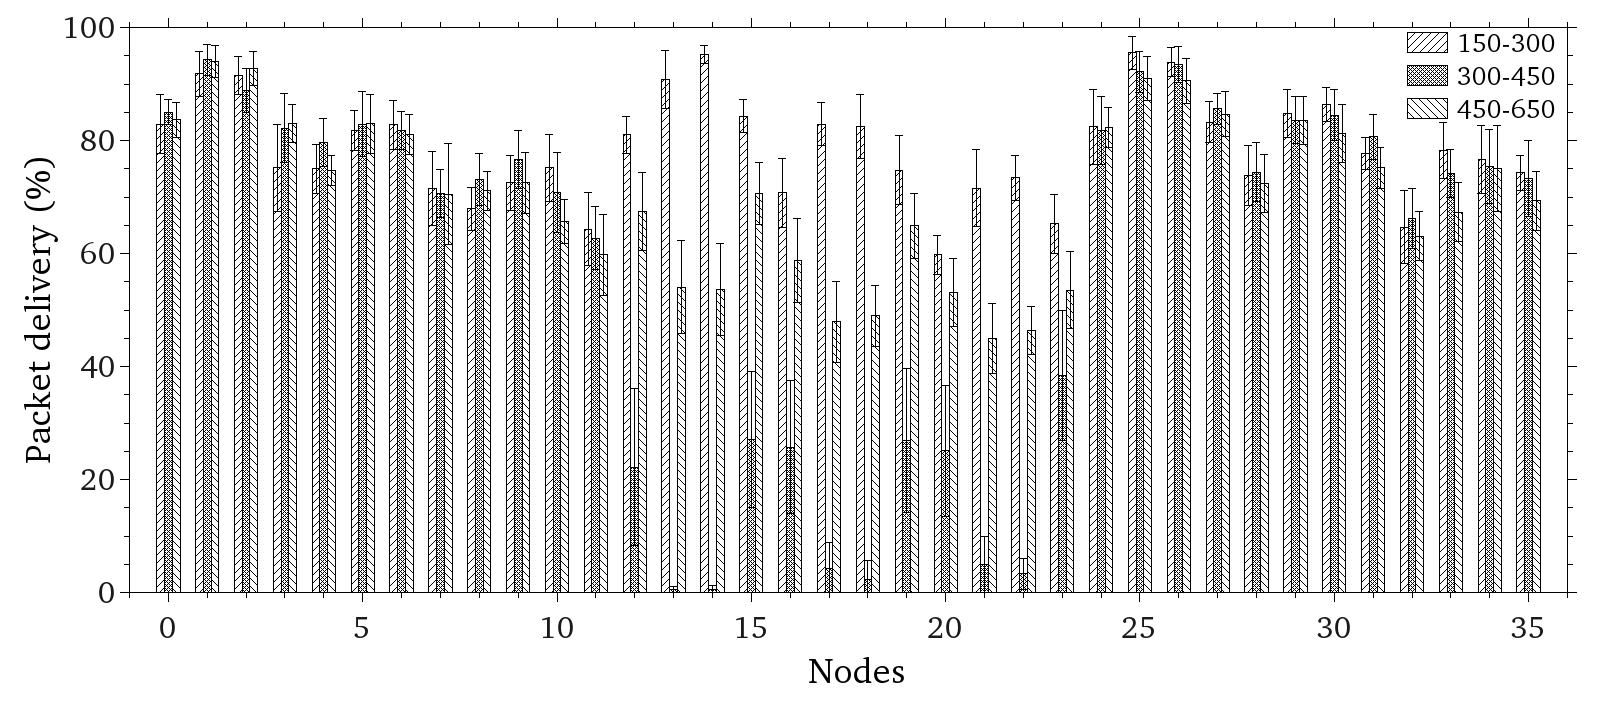
\includegraphics[scale=.21]{IEEE-consolidados/G-no-fases-mdap}}
\end{minipage}
\caption{Packet delivery in three periods: 150-300, 300-450 and 450-650.}
\label{fases}
\end{figure}


\section{Conclusion}






% if have a single appendix:
%\appendix[Proof of the Zonklar Equations]
% or
%\appendix  % for no appendix heading
% do not use \section anymore after \appendix, only \section*
% is possibly needed

% use appendices with more than one appendix
% then use \section to start each appendix
% you must declare a \section before using any
% \subsection or using \label (\appendices by itself
% starts a section numbered zero.)
%



% use section* for acknowledgement
\section*{Acknowledgment}


The authors would like to thank .....

This work is supported in part by CNPq, CAPES, FAPERJ, TBE/ANEEL and CELESC/ANEEL.


% Can use something like this to put references on a page
% by themselves when using endfloat and the captionsoff option.
\ifCLASSOPTIONcaptionsoff
  \newpage
\fi



% trigger a \newpage just before the given reference
% number - used to balance the columns on the last page
% adjust value as needed - may need to be readjusted if
% the document is modified later
%\IEEEtriggeratref{8}
% The "triggered" command can be changed if desired:
%\IEEEtriggercmd{\enlargethispage{-5in}}

% references section

% can use a bibliography generated by BibTeX as a .bbl file
% BibTeX documentation can be easily obtained at:
% http://www.ctan.org/tex-archive/biblio/bibtex/contrib/doc/
% The IEEEtran BibTeX style support page is at:
% http://www.michaelshell.org/tex/ieeetran/bibtex/
%\bibliographystyle{IEEEtran}
% argument is your BibTeX string definitions and bibliography database(s)
%\bibliography{IEEEabrv,../bib/paper}
%
% <OR> manually copy in the resultant .bbl file
% set second argument of \begin to the number of references
% (used to reserve space for the reference number labels box)
\bibliographystyle{IEEEtran}
\bibliography{./sbc-template}

% biography section
% 
% If you have an EPS/PDF photo (graphicx package needed) extra braces are
% needed around the contents of the optional argument to biography to prevent
% the LaTeX parser from getting confused when it sees the complicated
% \includegraphics command within an optional argument. (You could create
% your own custom macro containing the \includegraphics command to make things
% simpler here.)
%\begin{biography}[{\includegraphics[width=1in,height=1.25in,clip,keepaspectratio]{mshell}}]{Michael Shell}
% or if you just want to reserve a space for a photo:

\begin{IEEEbiography}[{\includegraphics[width=1in,height=1.25in,clip,keepaspectratio]{picture}}]{John Doe}
\blindtext
\end{IEEEbiography}

% You can push biographies down or up by placing
% a \vfill before or after them. The appropriate
% use of \vfill depends on what kind of text is
% on the last page and whether or not the columns
% are being equalized.

%\vfill

% Can be used to pull up biographies so that the bottom of the last one
% is flush with the other column.
%\enlargethispage{-5in}




% that's all folks
\end{document}



